\begin{frame}{The Reinforcement Learning Problem}
\begin{columns}
\column{0.5\textwidth}
\begin{itemize}
\item Deals with agents learning to take decisions in an environment that provides numerical rewards.
\item The goal of the agent is to maximize the cumulative reward obtained by interacting with environment
\end{itemize}

\column{0.5\textwidth}
\centering
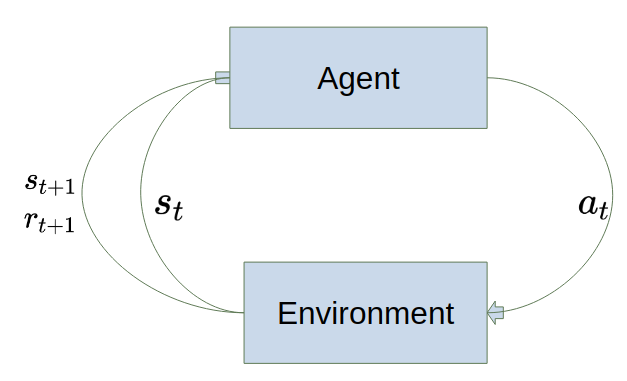
\includegraphics[scale = 0.25]{img/block.png}
\end{columns}
\end{frame}
\begin{frame}{Markov Decision Process (MDP)}
\begin{itemize}
    \item Mathematical Formulation of RL problem.
    \item Based on the \textbf{Markov property} which means that the current state completely captures the state of the world. More concretely:
    $P(s_{t+1}|s_t)$ = $P(s_{t+1}|s_t, s_{t-1}, ..., s_0)$ \item Defined by $(S, A, \mathbb{R},  \mathbb{P}, \gamma)$ 
    \begin{itemize}
        \item $S$ : set of possible states
        \item $A$ : set of possible actions
        \item $\mathbb{R}$ : distribution of reward given (state, action) pair. 
        \item $\mathbb{P}$ : transition probability which gives the distribution of next state given a (state, action) pair. 
        \item $\gamma$ : discount factor
    \end{itemize}
\end{itemize}
    
\end{frame}
\begin{frame}{Policy}
\begin{itemize}
    \item A policy describes the behavior of an agent.
    \item It is a function that maps state to action.
    \item Deterministic Policy:
        $a_t = \pi(s_t; \theta)$
    \item Stochastic Policy:
        $a_t \sim \pi(a_t|s_t;\theta)$
    \item The goal of an RL agent is to learn a policy which maximizes the agent’s cumulative discounted reward (also called return) which is defined as: $\sum_{t > 0}\gamma^{t-1}r_t$
\end{itemize}
\end{frame}
\begin{frame}{Value Functions} 
\begin{columns}
\column {0.5\textwidth}
\centering
\textbf{State Value Function}
\begin{itemize}
    \item A value function describes how good or bad a particular \textbf{state} is.
    \item It is defined by the expected cumulative reward starting from state $s_t$ and following a policy $\pi$.
    \newline
    $V_{\pi}(s_t) = \mathop{\mathbb{E}}_{\pi}[r_t + \gamma r_{t+1} + ... + \gamma^{T-t}r_{T} | s_t]$
    \item The optimal value function is defined as the maximum value function for all the policies.
    $V(s_t) = max_{\pi}(V_{\pi}(s_t))$
\end{itemize}
\column {0.5\textwidth}
\centering
\textbf{Action Value Function}
\begin{itemize}
    \item Describes how good a \textbf{state, action} pair is.
    \item It is defined as the expected cumulative reward obtained on starting from a state $s_t$, taking action $a_t$ and then following a policy $\pi$
    \newline
    $Q_{\pi}[s_t,a_t] =\mathop{\mathbb{E}}_{\pi}[r_t + \gamma r_{t+1} + ... + \gamma^{T-t}r_{T} | s_t, a_t] $
    \item The optimal Q value function can be defined as the maximum of q value functions for all the policies.
    $Q(s_t, a_t) = max_{\pi}(Q_{\pi}(s_t, a_t))$
\end{itemize}
\end{columns}
    
\end{frame}
\begin{frame}{Solving the RL Problem}
\begin{itemize}
    \item Value based RL
    \begin{itemize}
        \item Learn optimal action value function $Q$
        \item Policy is the generated implicitly from the learned $Q$ function (greedy, $\epsilon$ greedy)
        \item Eg: Q Learning, SARSA, Monte Carlo Control etc.
    \end{itemize}
    \item Policy based RL (Policy Gradient Methods)
    \begin{itemize}
        \item Learn the policy $\pi$ directly.
        \item Eg: REINFORCE , A2C, TRPO, PPO, DDPG etc.   
    \end{itemize}
\end{itemize}
    
\end{frame}
